%!TEX root = paper.tex
In this section, I discuss the implications of the model by constructing three counterfactuals.
First,
I examine whether the fiscal competition characterized by the model can improve
allocation efficiency by changing the locations of firms. Second, I analyze the potential impacts
of suppressing the fiscal competition between city governments on industrial land prices and fiscal
revenues. Third, I discuss the potential impacts of rising urban wages on the fiscal competition.

\subsection{Allocation efficiency}
As I discussed in \Cref{sec:intro} and \Cref{sec:institution}, the potential benefits
of fiscal competition between cities is the improvement of resource allocation between cities.
More specifically, cities that are disadvantaged in attracting firms (wage levels are high
in these cities) can increase the probability of landing the firms by decreasing the land price more
sharply than their competitors. But the extent of these benefits is unclear, since the sharp decreases
of prices by disadvantaged cities may also promote other cities to decrease their prices,
and probabilities of getting
the firm across cities may not change by a lot.

To measure the exact impact of fiscal competition, I consider the counterfactual that the
central government freezes the industrial land market by fixing the industrial land price
across the whole country. If the land price is fixed,
the city with the lowest wage level
among the candidates of a firm
will have the highest probability of landing the firm.
And I denote these cities as advantaged cities.

I use the change of the probabilities of the advantaged cities landing the firms
to measure the impact of fiscal competition on allocation efficiency.
If fiscal competition decreases these probabilities significantly,
the disadvantaged cities will have higher chances to get the firms,
i.e., fiscal competition may be helpful to improve allocation efficiency.

I also do thirty simulations for both fiscal competition and fixed land price cases, and
the empirical distribution of the probability of getting the firm in the fixed land price case is shown
with the baseline case together
in the \Cref{fig: allocation efficiency}.
\begin{figure}[H]
    \centering
    \caption{The empirical CDF of the probability of getting the firm for advantaged cities}
    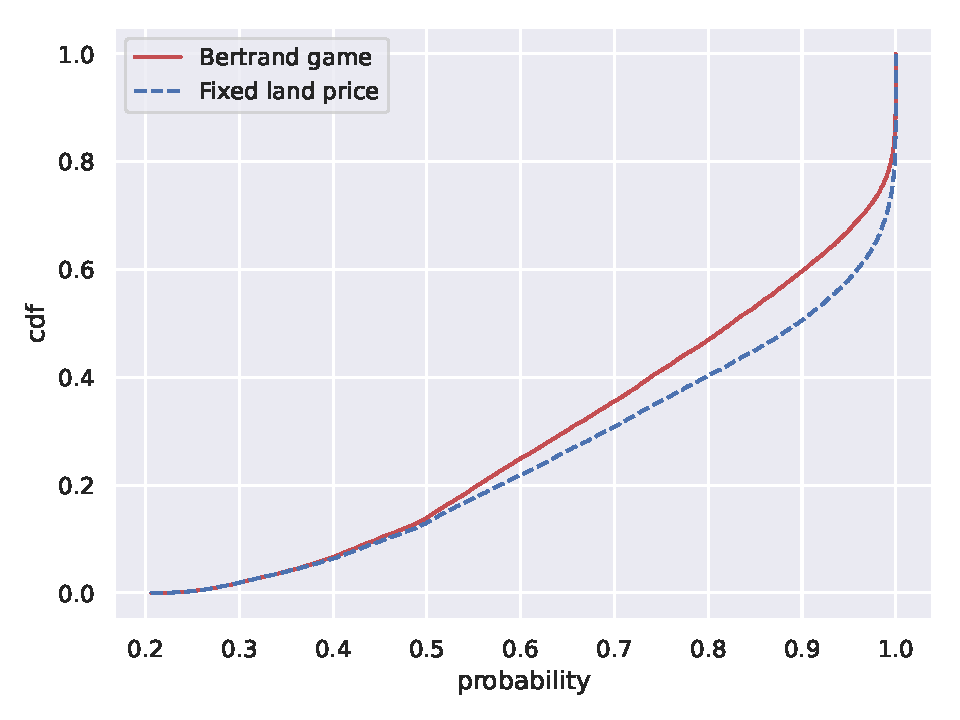
\includegraphics[scale=0.6]{\graphs/allocation_efficiency.pdf}
    \fnote{Notes: I use the preferred estimates to do thirty simulations,
        and calculate all the choice probabilities in the $N \times S ~(1019 \times 30)$
        location choice problems
        to draw the empirical distribution.}
    \label{fig: allocation efficiency}
\end{figure}

I compare the empirical CDF of the highest probability
of getting the firm in the Bertrand game with which
in the case of nationwide fixed land price (see \Cref{fig: allocation efficiency}),
and they are very similar,
though the empirical CDF curve of the Bertrand game is slightly higher than which
of the fixed land price case, i.e. the highest probability in the Bertrand game is
stochastically dominated by that in the fixed land price case.
This implies that
the impact of fiscal competition on the locations of firms (allocation efficiency) is very small
though fiscal competition indeed gives some disadvantaged cities higher chances
of landing the firms.

I also show the descriptive statistics of the
probability of getting the firms for advantaged cities in
\Cref{table: allocation_efficiency} below. It shows that
fixing the land price (banning the fiscal competition) will increase this probability by
2.9\% on average and 7\% for the median,
which verifies again that the impact of fiscal competition on allocation efficiency is small.
\begin{table}[H]
\centering
\caption{Empirical distribution of probability of getting the firms for advantaged cities}
\label{table: allocation_efficiency}
\begin{tabular}{lccc}
\toprule
 & fixed land price & Bertrand game & difference \\
\midrule
mean & 0.801 & 0.773 & 0.029 \\
std & 0.218 & 0.215 & 0.002 \\
min & 0.206 & 0.206 & 0.000 \\
25\% percentile & 0.635 & 0.601 & 0.035 \\
median & 0.895 & 0.825 & 0.071 \\
75\% percentile & 0.996 & 0.984 & 0.012 \\
max & 1.000 & 1.000 & 0.000 \\
\bottomrule
\end{tabular}
\end{table}



\subsection{Potential impacts of fiscal centralization}
As I discussed in \Cref{subsec:discussion of results}, the estimates of $\hat{\beta} = \estbeta$
is much greater than the official tax revenue share. Such large city governments'
revenue share of firms' output reflects not only the strong incentive of
local officials to attract firms, but also the significant economic and fiscal power of
local officials, which can convert the spillover effects of industrial firms on local businesses,
the housing market, etc., to their fiscal revenue. Moreover, as \cite{kroeber2020china} observed:
\textit{``The ability of these leaders (local officials) to act independently
    of central dictates, and in response to local needs, has contributed to China's
    resilience and dynamism.''}. However, the fierce fiscal competition between local
governments due to this ability may also waste a lot of potential fiscal revenue
in the industrial land market as I discussed before.

The autonomy of local officials in economic affairs declines significantly after 2013
due to the re-centralization of the governance structure in China and the anti-corruption movement,
and I call this change ``fiscal centralization'' reflected by the decrease of $\beta$.

I examine the potential impacts of the decrease of $\beta$ by counterfactual experiments. Specifically,
I decrease the estimated $\hat{\beta}$ by 10\%, 25\%, 50\% respectively, and do thirty simulations to
observe the change in the average land price, total land selling revenue
and total fiscal revenue across all firms in the data set.

The change of land price distribution is shown in \Cref{fig: decrease of beta},
which draws the land price distribution across all firms for the original estimates $\beta = \estbeta$,
$\beta = 0.405$ (10\% decrease), $\beta = 0.338$ (25\% decrease), and $\beta=0.225$ (50\% decrease).

\begin{figure}[H]
    \centering
    \caption{Change of land price distribution due to decrease of $\beta$}
    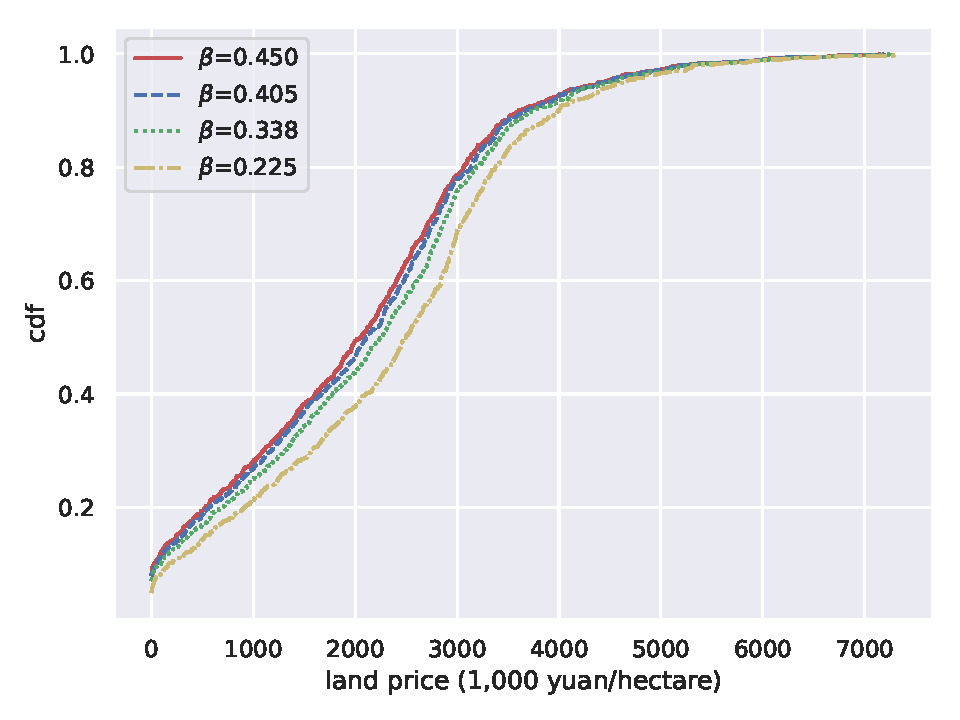
\includegraphics[scale=0.6]{\graphs/cdf_beta_decrease.pdf}
    \fnote{Notes: The estimates $\hat{\beta} = \estbeta$. $\beta = 0.414, ~0.345, ~0.230$
        are equivalent to 10\%, 25\%, 50\% decrease of $\hat{\beta}$ respectively.
        For each $\beta$, I do 30 simulations for each firm to draw the empirical CDF plot.}
    \label{fig: decrease of beta}
\end{figure}

The figure shows that as $\beta$ decreases, the empirical CDF curve of land price shifts to the right,
which means more lands are sold at higher prices as $\beta$ decreases. However,
for $\beta = 0.405$ and $\beta = 0.338$, the empirical CDFs are close to the baseline
($\beta = \estbeta$). Thus, the impact of fiscal centralization on land prices is limited.


The reason behind this change of price distribution is reflected by the trade-off between
land-selling revenue and the fiscal revenue generated by landing the firm, which is characterized
by \eqref{gov revenue}. Intuitively, as the governments' revenue share of firms'
output $\beta$ decreases, the expected fiscal revenue of attracting firms using low land prices
also decrease. Thus, the local officials care more about
land-selling revenue even though higher land prices will decrease their probability of
getting the firms. However, even if $\beta$ decreases by 25\%, the spillover effects of
attracting firms are still sufficiently large, as I discussed in
\Cref{subsec:discussion of results}.
Thus, the rise of land prices is limited.

I also calculate the percent changes in the average land price, total land selling revenue, and
total fiscal revenue at different values of $\beta$, and the results are shown in
\Cref{table: decrease_beta}. It shows
the average land price and total land selling revenue increase as $\beta$ decreases, but
the increase is not large compared to the decrease of $\beta$.
However, I also notice that the total fiscal revenue, which is the summation of
total land selling revenue and total output share decreases sharply as $\beta$ decreases.
This is because the land-selling revenue constitutes only a small proportion of
the total fiscal revenue compared to the huge revenue generated by landing firms.
\begin{table}[H]
\centering
\caption{The impacts of decrease in $\beta$}
\label{table: decrease_beta}
\begin{tabular}{ccccc}
\toprule
$\beta$ & change of $\beta$ & average land price & total land selling revenue & total fiscal revenue \\
\midrule
0.405 & -10\% & 2.52\% & 1.99\% & -8.99\% \\
0.338 & -25\% & 7.16\% & 5.65\% & -22.43\% \\
0.225 & -50\% & 17.38\% & 14.04\% & -44.62\% \\
\bottomrule
\end{tabular}
\end{table}


To conclude my discussion in this subsection, the trend of fiscal centralization
after 2013 might restrict the fiscal competition between local governments and increase
the industrial land price if the total output level across the nation is stable.
However, the increase in land price is limited, and
the loss of fiscal revenue due to the decrease in local governments' output
share is difficult to be compensated by the increasing industrial land-selling revenue.
Thus, fiscal centralization poses challenges for the central government in how to
compensate the local governments' potential fiscal revenue loss.

\subsection{Potential impacts of the rising wage level}
In recent years, the impacts of rising urban wages on China's economy are intensely discussed in
both economic literature and public policy debates. The rising urban wage in China after the late 2000s
is caused by the rural surplus labor crossing the Lewisian turning point
\citep{cai2010growth} and the age structure change of population \citep{fang2016china}.
I am particularly interested in the potential impacts of the rising urban wage
on the fiscal competition between city governments
since labor and land are both inputs in the firm's production function.

To implement the counterfactual analysis, I increase the wage level in all cities
by 10\%, 25\%, and 50\% respectively,
and examine the impacts on average land price, total land selling revenue, total fiscal revenue
by simulations.

I draw the empirical distributions of industrial land price under different rises of wage
in \Cref{fig: increase_wage}. As \Cref{fig: increase_wage}
shows, the new empirical CDF curves of land price
are close to the baseline if wage increases by 10\% or 25\% in all cities.
If the wage level rises by 50\% in all cities,
the distribution shifts to the right more clearly.
Nevertheless, all three cases show that the average land price is higher
if the wage level increases in all cities.

\begin{figure}[H]
    \centering
    \caption{Change of land price distribution due to increase of wage}
    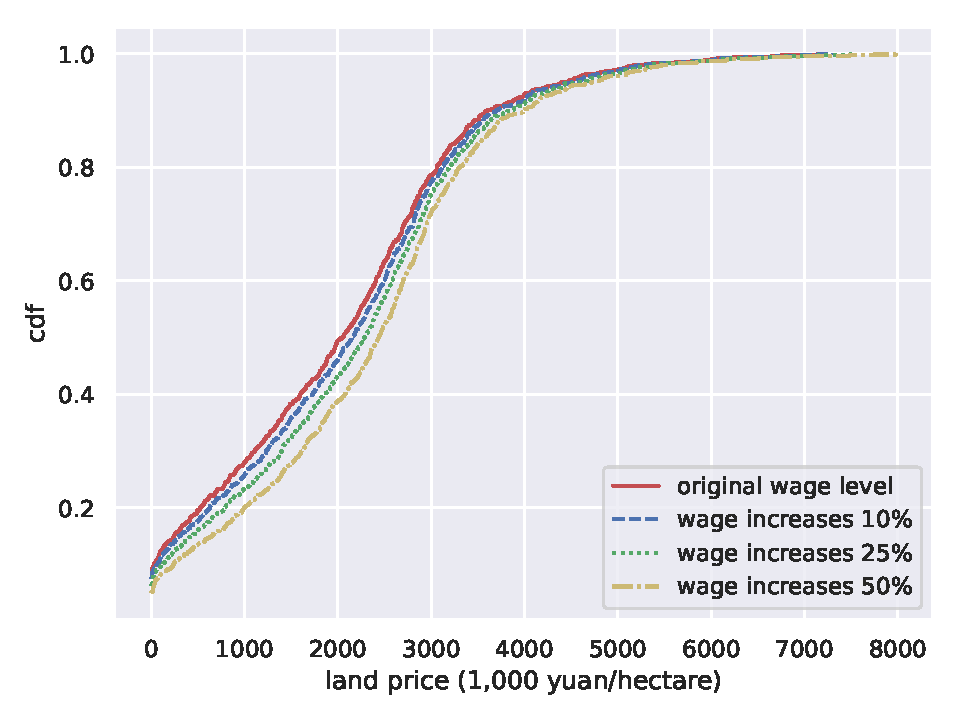
\includegraphics[scale=0.6]{\graphs/cdf_wage_increase.pdf}
    \fnote{Notes: The preferred estimates are used in all four cases.
        I do thirty simulations for each firm to draw the empirical CDF plots.}
    \label{fig: increase_wage}
\end{figure}

The intuition behind the rise of average land price as wage level increases in the whole nation is
that labor and land are both inputs in the firm's production function,
and the national-wide wage increase will make the relative price of labor to land
more expensive than before. In other words,
firms will be more sensitive to labor costs in their location choice problem than before, and
city governments will raise the land price since firms are not as sensitive to land prices as before.

I also show the impacts of the increase in wage on average land price, total land selling revenue,
and total fiscal revenue in \Cref{table: increase_wage}.
The average land price increases as the wage level increases, but the increase is not sharp.


\begin{table}[H]
\centering
\caption{The impacts of rising wage level}
\label{table: increase_wage}
\begin{tabular}{ccccc}
\toprule
wage increase & average land price & total land selling revenue & total fiscal revenue \\
\midrule
10.00\% & 3.97\% & 5.37\% & 0.45\% \\
25.00\% & 9.23\% & 12.60\% & 1.06\% \\
50.00\% & 16.53\% & 22.98\% & 1.93\% \\
\bottomrule
\end{tabular}
\end{table}


To conclude my discussion in this subsection, I find that the rising urban wage would
increase the average industrial land price in China, i.e. restrict the fiscal
competition, but just to a small extent. This implies it is difficult to change
the pattern of fiscal competition by the change of production factor prices (pure market power).















